\subsection{Architektura}

Cílem práce je vytvořit komplexní aplikaci, která využívá zařízení s větší obrazovkou jako prostředí pro běh hry, tzv. frontend, a mobilní telefon jako oddělený ovládací prvek (kontrolér). \par
Z tohoto rozdělení úkolů pak vychází základní nároky na architekturu systému skládající se z kontrolérové části (mobilní aplikace), zobrazovacího frontendu (webová aplikace) a serverového backendu, který musí zastat většinu funkcionality, – především tedy autentizaci uživatelských zařízení (frontend i kontrolér) a jejich spárování, komunikaci s nimi, analýzu zaslaného obrazu, vykonávání analyzovaného uživatelského kódu a zprostředkování výsledků pro frontend. Samozřejmými součástmi a podsystémy jsou pak databázová část, emailová komunikace či cachování (vyžívání dočasné vyrovnávací paměti). Architekturu názorně shrnuje schéma na obr. \ref{fig:architektura}

\begin{figure}[h]
    \centering
    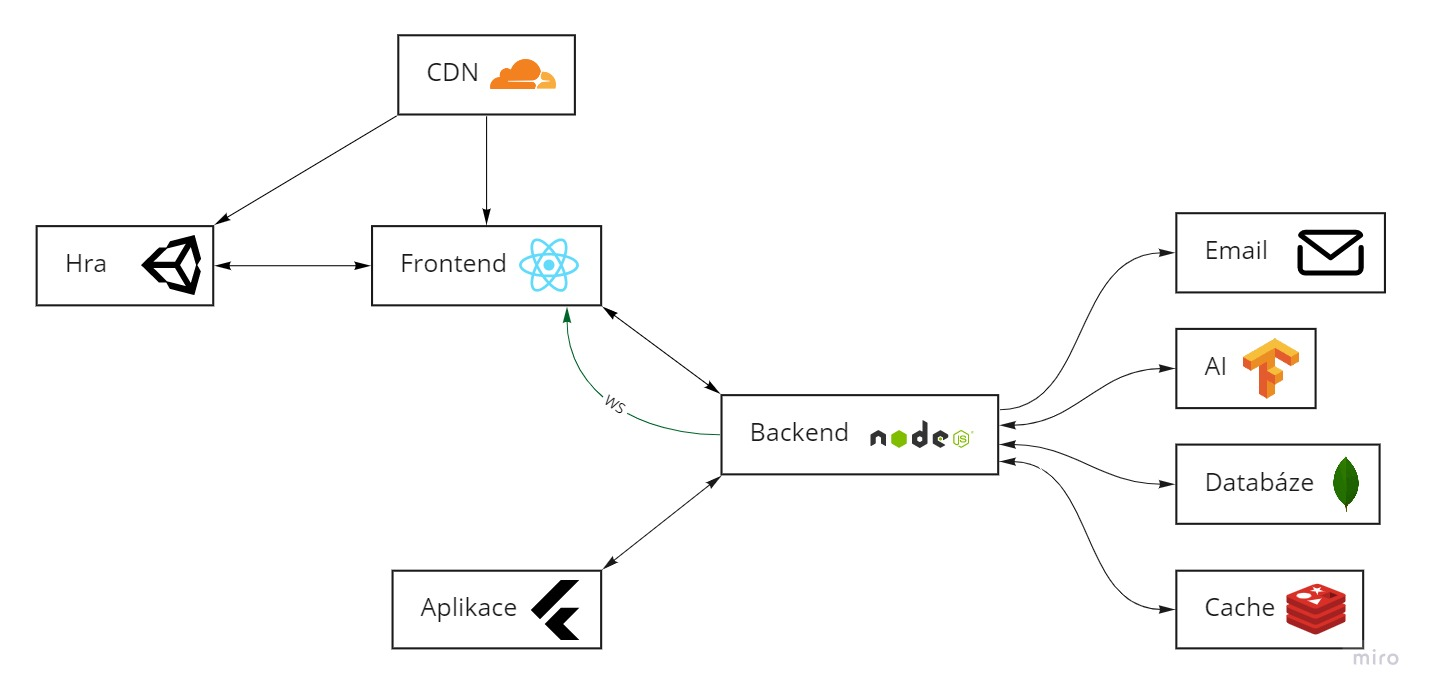
\includegraphics[width=0.6\textwidth]{img/architektura.jpg}
    \caption{Architektura aplikace.}
    \label{fig:architektura}
\end{figure}